%%
%% Copyright (c) 2018 The Authors.  All Rights Reserved.
%%
%% Weitian LI, et al.
%% School of Physics and Astronomy, Shanghai Jiao Tong University,
%% Shanghai, China.
%%
%% 2018-08-23
%%

\documentclass[letters,a4paper,fleqn,usenatbib]{mnras}
% Available options:
% - letters : for papers in the journal's Letters section (<=5 pages)
% - onecolumn : single column
% - doublespacing : double line spacing (do NOT submit in this format)
% - usenatbib : (always use this) use `natbib' package for citations
% - usegraphicx : includes the `graphicx' package
% - useAMS : support 3 upright Greek characters
% - usedcolumn : use `dcolumn' package for table column alignment

% Chinese
\usepackage{xeCJK}
\setCJKmainfont{Noto Serif CJK SC}[BoldFont=Noto Sans CJK SC]
\setCJKsansfont{Noto Sans CJK SC}

\usepackage{newtxtext,newtxmath}
\usepackage[T1]{fontenc}
\usepackage{ae,aecompl}

%
% Custom packages
%
\usepackage{graphicx}
\usepackage{amsmath}
\usepackage{amssymb}
\usepackage{siunitx}  % typeset units; from `texlive-science'

\graphicspath{{./}{figures/}}  % NOTE: the trailing '/' matters

\sisetup{
  range-phrase=\text{--},
  range-units=single,
  product-units=repeat,
  list-separator={, },
  list-final-separator={, and },
  separate-uncertainty=true,
}
\DeclareSIUnit\MHz{\mega\hertz}
\DeclareSIUnit\kHz{\kilo\hertz}
\DeclareSIUnit\jansky{Jy}
\DeclareSIUnit\mJy{\milli\jansky}

\def\sectionautorefname{Section}
\def\subsectionautorefname{Section}
\def\figureautorefname{Fig.}
\def\tableautorefname{Table}

%
% Custom commands
%
\newcommand{\R}[1]{\mathrm{#1}}
\newcommand{\B}[1]{\mathbfit{#1}}
\newcommand{\M}[1]{\mathbfss{#1}}


%%======================================================================
%% Title page
%%

%      ............................................. (<=45 chars)
\title[EoR Separation with CDAE]{%
  Deep-learning-based Method to Separate the EoR Signal
  Using the Convolutional Denoising Autoencoder
}

% If you need two or more lines of authors, add an extra line using \newauthor
\author[Li~et~al.]{%
Weitian Li,$^{1}$\thanks{E-mail:
  \href{mailto:liweitianux@sjtu.edu.cn}{liweitianux@sjtu.edu.cn} (WL);
  \href{mailto:hgxu@sjtu.edu.cn}{hgxu@sjtu.edu.cn} (HX)}
Haiguang Xu,$^{1,2,3}$\footnotemark[1]
Zhixian Ma,$^{4}$
Ruimin Zhu,$^{5}$
Dan Hu,$^{1}$
Zhenghao Zhu,$^{1}$
\newauthor
Chenxi Shan,$^{1}$
Jie Zhu$^{4}$
and
Xiang-Ping Wu$^{6}$
\\
% List of institutions
$^{1}${School of Physics and Astronomy,
  Shanghai Jiao Tong University,
  800 Dongchuan Road, Shanghai 200240, China} \\
$^{2}${Tsung-Dao Lee Institute,
  Shanghai Jiao Tong University,
  800 Dongchuan Road, Shanghai 200240, China} \\
$^{3}${IFSA Collaborative Innovation Center,
  Shanghai Jiao Tong University,
  800 Dongchuan Road, Shanghai 200240, China} \\
$^{4}${Department of Electronic Engineering,
  Shanghai Jiao Tong University,
  800 Dongchuan Road, Shanghai 200240, China} \\
$^{5}${Department of Statistics,
  Northwestern University,
  2006 Sheridan Road, Evanston, IL 60208, US} \\
$^{6}${National Astronomical Observatories,
  Chinese Academy of Sciences,
  20A Datun Road, Beijing 100012, China}
}

% These dates will be filled out by the publisher
\date{Accepted XXX. Received YYY; in original form ZZZ}

% Enter the current year, for the copyright statements etc.
\pubyear{2018}

% Don't change these lines
\begin{document}
\label{firstpage}
\pagerange{\pageref{firstpage}--\pageref{lastpage}}
\maketitle

%
% Abstract
% (<=200 words for Letters)
%
\begin{abstract}
The overwhelming foreground contamination is one of the primary
challenge in measuring the \SI{21}{\cm} signal to probe the EoR.
Although the foreground is expected to be spectrally smooth,
the frequency-dependent beam effects of interferometers can
seriously damage the smoothness of foreground spectrum,
imposing great difficulties on existing foreground removal methods.
In this work, we propose a novel deep-learning-based method by employing
the convolutional denoising autoencoder (CDAE) to separate the EoR signal.
The proposed CDAE, which consists of a 7-layer encoder, a 7-layer
decoder, and one output layer, is simple but powerful and successfully
learns robust features of the faint EoR signal that is contaminated by the
severe foreground emission.
By training and evaluating the CDAE on the simulated SKA images, it
achieves excellent performance with the correlation coefficient between
the separated EoR signal and the simulated `true' signal being
$\rho_{\R{cdae}} = \num{0.985 +- 0.009}$.
As a comparison, the traditional polynomial fitting method has very poor
performance ($\rho_{\R{pfit}} = \num{0.241 +- 0.103}$ on the same data set).
In conclusion, our deep-learning-based method can accurately separate
the faint EoR signal in the presence of severe foreground contamination
and complicated instrumental effects.
\end{abstract}

% Select between one and six entries from the list of approved keywords.
% Don't make up new ones.
% https://academic.oup.com/DocumentLibrary/mnras/keywords.pdf
\begin{keywords}
methods: data analysis --
techniques: interferometric --
dark ages, reionization, first stars --
radio continuum: general
\end{keywords}


%%======================================================================
%% Paper body
%%

\section{Introduction}
\label{sec:intro}

The \SI{21}{\cm} line emission of the neutral hydrogen,
which is believed to be redshifted to frequencies below \SI{200}{\MHz},
is regarded as a decisive probe to directly explore the epoch of
reionization (EoR), a period of the early Universe
($z \sim \numrange{6}{15}$) that is still poorly understood
\citep[see][for reviews]{furlanetto2006rev,furlanetto2016rev}.
As of today, several low-frequency radio interferometers have been built
or under construction to target the \SI{21}{\cm} signal, including
21CMA \citep{zheng2016}, GMRT \citep{paciga2011}, MWA \citep{tingay2013},
LOFAR \citep{vanHaarlem2013}, PAPER \citep{parsons2010},
HERA \citep{deboer2017}, and SKA \citep{koopmans2015rev}.
The observational challenges, however, are immense due to a variety of
complicated instrumental effects, ionospheric distortions, radio frequency
interference, and the strong astronomical foreground contamination that
overwhelms the EoR signal by about \numrange{4}{5} orders of magnitude
\citep[see][for a review]{morales2010rev}.

Fortunately, in the frequency dimension, the foreground contamination
is expected to be very smooth, while the EoR signal fluctuates rapidly
on scales of $\lesssim \si{\MHz}$.
This important difference is the key characteristic exploited by many
foreground removal methods in order to uncover the faint EoR signal,
including
parametric fitting methods \citep[e.g.,][]{wang2006,liu2009fgrm,wang2013}
and non-parametric methods \citep[e.g.,][]{harker2009,chapman2013,mertens2018}.

However, the frequency-dependent beam effects can damage the smoothness
of the foreground spectra \citep{liu2009ps}.
The point spread function (PSF), which is the Fourier Transform (FT)
of the interferometer layout, varies with observing frequencies and
has jagged side-lobes extending far beyond the main lobe due to the
incomplete $uv$ coverage.
Therefore, an unresolved or mis-subtracted source can leave residuals
at different positions in the cleaned images of different frequencies.
As a result, every pixel in the obtained image cube has unpredictable
oscillating residuals along the frequency dimension, imposing great
difficulties on the foreground removal methods that rely on the
smoothness of the foreground contamination \citep[see also][]{liu2009ps}.

Given the complicated profiles and frequency-dependent variations of
the PSF, it is extremely difficult to craft a parametric model for
existing foreground removal methods to overcome the intricate beam
effects, thus the data-driven modelling method is more feasible and
appealing [这主要是我们自己的观点、未找到相关文献可引].
In recent years, the deep learning algorithms have seen prosperous
developments and brought breakthroughs into a variety of fields, such
as image classification, speech recognition, and object detection
\citep[see][for a recent review]{lecun2015}.
Among all kinds of neural network architectures, the autoencoder
is able to learn robust features in the data \citep{vincent2008}
and has been widely applied to
dimensionality reduction \citep{hinton2006},
image inpainting and denoising \citep{suganuma2018},
speech separation \citep{grais2017}, and so on.

In this paper, in order to tackle the intricate frequency-dependent
beam effects, we propose a novel deep-learning-based method to separate
the EoR signal along the frequency dimension by making use of the
convolutional denoising autoencoder (CDAE), a popular variant of
autoencoders that is designed to recover the original clean signal
from the noisy data.
To the best of our knowledge, there is no similar deep-learning-based
methods for the EoR signal separation in the literature.
In \autoref{sec:method}, we briefly introduce the CDAE and elaborate
the proposed method.
In \autoref{sec:experiments}, we demonstrate the performance of the
method by applying it to the simulated SKA images.
We discuss the method and carry out a comparison to the traditional
polynomial fitting method in \autoref{sec:discussions}.
Finally, we conclude our work in \autoref{sec:conclusions}.
The implementation code and data are made public at
\url{https://github.com/lwieitianux/cdae-eor}.


%%======================================================================
\section{Methodology}
\label{sec:method}

%%----------------------------------------------------------------------
\subsection{Convolutional denoising autoencoder}
\label{sec:cdae}

An autoencoder is composed of two parts: the encoder and the decoder,
which can be described by two functions $f(\cdot)$ and $g(\cdot)$,
respectively.
The encoder maps the input $\B{x}$ to an internal code $\B{h}$, i.e.,
$\B{h} = f(\B{x})$, while the decoder tries to reconstruct the input
from the code $\B{h}$, i.e., $\B{r} = g(\B{h})$.
By placing constraints (e.g., dimensionality, sparsity) on the
internal code $\B{h}$ and training the autoencoder to minimise the
loss $L(\B{x}, \B{r})$, which quantifies the difference between the
reconstruction $\B{r}$ and the input $\B{x}$, the autoencoder is able
to learn the codes that effectively represent the input data
\citep[chapter 14]{goodfellow2016}.

The CDAE combines the ideas of both the convolutional neural network
and the denoising autoencoder \citep{du2017}.
The use of multiple convolutional layers improves the ability of the
CDAE to extract sophisticated features in the data \citep{masci2011}.
Training the CDAE on the noisy data $\B{\~{x}}$ forces the CDAE to
learn features that are robust to the noise in the data, thus the
trained CDAE can recover the original data $\B{x}$ from the noisy
input $\B{\~{x}}$ \citep{vincent2008,vincent2010}.

In the task of separating the EoR signal, the foreground contamination,
albeit very strong, can be regarded as the noise that corrupts the
target signal.
Therefore, the CDAE is the appropriate deep-learning method to extract
the features of the faint EoR signal that are robust to the foreground
contamination and the frequency-dependent beam effects.


%%----------------------------------------------------------------------
\subsection{Network architecture}
\label{sec:architecture}

We follow the common practice to build the CDAE architecture
\citep[e.g.,][]{suganuma2018,geron2017}.
The encoder and decoder parts are symmetric and use the exponential
linear unit (ELU) as the activation function \citep{clevert2016},
while the output layer uses the `tanh' activation function (see also
\autoref{sec:preprocessing}).
The batch normalisation is applied to all layers except for the output
layer to improve the training process as well as to act as a regularizer
to prevent overfitting \citep{ioffe2015}.
The filters in all layers are of size 3 and one-dimensional (1D) because
the CDAE input is a 1D vector representing one sky pixel along the
observing frequency dimension.

We have evaluated multiple CDAE architectures of different number of
layers and filters.
The simplest one with sufficiently good performance is selected, as
shown in \autoref{fig:network}.
The chosen CDAE consists of a 4-layer encoder with $(32,64,64,32)$
filters, a 4-layer decoder with $(32,64,64,32)$ filters, and one output
layer.
We also note that a simpler CDAE is less likely to overfit the data
and can be more easily extended and applied to the forthcoming EoR
experiments.

\begin{figure}
  \centering
  \includegraphics[width=0.8\columnwidth]{network-crop}
  \caption{\label{fig:network}%
    The network architecture of the proposed CDAE, consisting of a
    4-layer encoder (the orange boxes), a 4-layer decoder (the blue
    boxes), and one output layer (the green box).
    The layers in the encoder and decoder use the ELU activation
    function and batch normalisation (BN), while the output layer uses
    the `tanh' activation function.
    All filters are of size 3 and the number of filters in each layer
    is marked in the braces.
  }
\end{figure}


%%----------------------------------------------------------------------
\subsection{Training and evaluation}
\label{sec:train-eval}

The CDAE is initialised by the He uniform initialiser \citep{he2015}
and is trained using the Adam optimisation method \citep{kingma2015}.
The loss, which describes the difference between the output of the CDAE
and the `true' data, is calculated as the `mean squared error' (MSE),
i.e.,
\begin{equation}
  \label{eq:loss}
  L = \frac{1}{N_{\R{ds}}} \sum_{i=1}^{N_{\R{ds}}}
    \left[ \B{s}_o^{(i)} - \B{s}_t^{(i)} \right]^T
    \left[ \B{s}_o^{(i)} - \B{s}_t^{(i)} \right],
    \quad i = 1, 2, \cdots, N_{\R{ds}},
\end{equation}
where
$\B{s}_o$ and $\B{s}_t$ are column vectors representing the separated
and the simulated `true' EoR signal, respectively,
and $N_{\R{ds}}$ is the number of data points in the data set.
By training the CDAE to minimise the loss, the CDAE is able to predict
the `true' data from the noisy input.

To evaluate the performance of the CDAE in separating the EoR signal,
the commonly used Pearson's correlation coefficient
\citep[e.g.,][]{harker2009,chapman2013}
is adopted to measure the similarity between the separated EoR signal
$\B{s}_o$ and the `true' signal $\B{s}_t$:
\begin{equation}
  \label{eq:corrcoef}
  \rho(\B{s}_o, \B{s}_t) =
    \frac{\sum_{j=1}^{n}(s_{o,j}-\bar{s}_p)(s_{t,j}-\bar{s}_t)}{
      \sqrt{\sum_{j=1}^{n}(s_{o,j}-\bar{s}_p)^2
        \sum_{j=1}^{n}(s_{t,j}-\bar{s}_t)^2}
    },
\end{equation}
where $\bar{s}_o$ and $\bar{s}_t$ are the mean values.
The closer the correlation coefficient is to one, the better the
performance of separation.


%%======================================================================
\section{Experiments}
\label{sec:experiments}

%%----------------------------------------------------------------------
\subsection{Simulation of the SKA images}
\label{sec:simulation}

We carry out end-to-end simulations to generate the SKA images for
training the proposed CDAE and evaluating the performance.
We choose the \SI{8}{\MHz} frequency band centred at \SI{158}{\MHz} as
an example, which is divided into 101 channels of width \SI{80}{\kHz}.
Following the approach described in detail in our previous works
\citep{wang2010,wang2013}, we simulate the sky maps of the foreground
emission contributed by the Galactic synchrotron and free-free
emissions, extragalactic point sources (the bright ones with a
\SI{158}{\MHz} flux density $S_{158} > \SI{10}{\mJy}$ are assumed to
have been removed; e.g., \citealt{liu2009ps}), and radio haloes.
The sky maps of the EoR signal are created using the `faint galaxies'
data set released by the Evolution Of 21~cm Structure project
\citep{mesinger2016}.
The maps cover a sky patch of size \SI{10 x 10}{\degree} and have
a pixel size of \SI{20}{\arcsecond} (i.e., \num{1800 x 1800} pixels).

To fully take into account the frequency-dependent beam effects of
interferometers, the SKA1-Low layout configuration\footnote{%
  SKA1-Low Configuration Coordinates:
  \url{https://astronomers.skatelescope.org/wp-content/uploads/2016/09/SKA-TEL-SKO-0000422_02_SKA1_LowConfigurationCoordinates-1.pdf}
  (released on 2016 May 21)}
is employed in the \textsc{oskar}\footnote{%
  OSKAR: \url{https://github.com/OxfordSKA/OSKAR} (version 2.7.0)}
simulator \citep{mort2010} to perform the simulated observations for the
above sky maps.
The visibility data are then imaged by the \textsc{wsclean}\footnote{%
  WSClean: \url{https://sourceforge.net/p/wsclean} (version 2.5)}
imager \citep{offringa2014} using the natural weighting and baseline
range of \numrange{30}{1000} wavelengths in order to emphasise the
faint diffuse EoR signal, and the created images are cropped to keep
only the central \SI{2 x 2}{\degree} regions (i.e., \num{360 x 360}
pixels).
Therefore, we obtain two image cubes of size \num{360 x 360 x 101}
for the EoR signal ($\M{C}_{\R{eor}}$) and the foreground emission
($\M{C}_{\R{fg}}$), respectively.
An example spectrum and the corresponding differential spectrum for
the foreground emission are shown in \autoref{fig:simudata}.
It is clearly shown that, compared with the original spectrum without
instrument observation (the top panel), the smoothness of the foreground
spectrum is seriously damaged by the frequency-dependent beam effects.

\begin{figure}
  \centering
  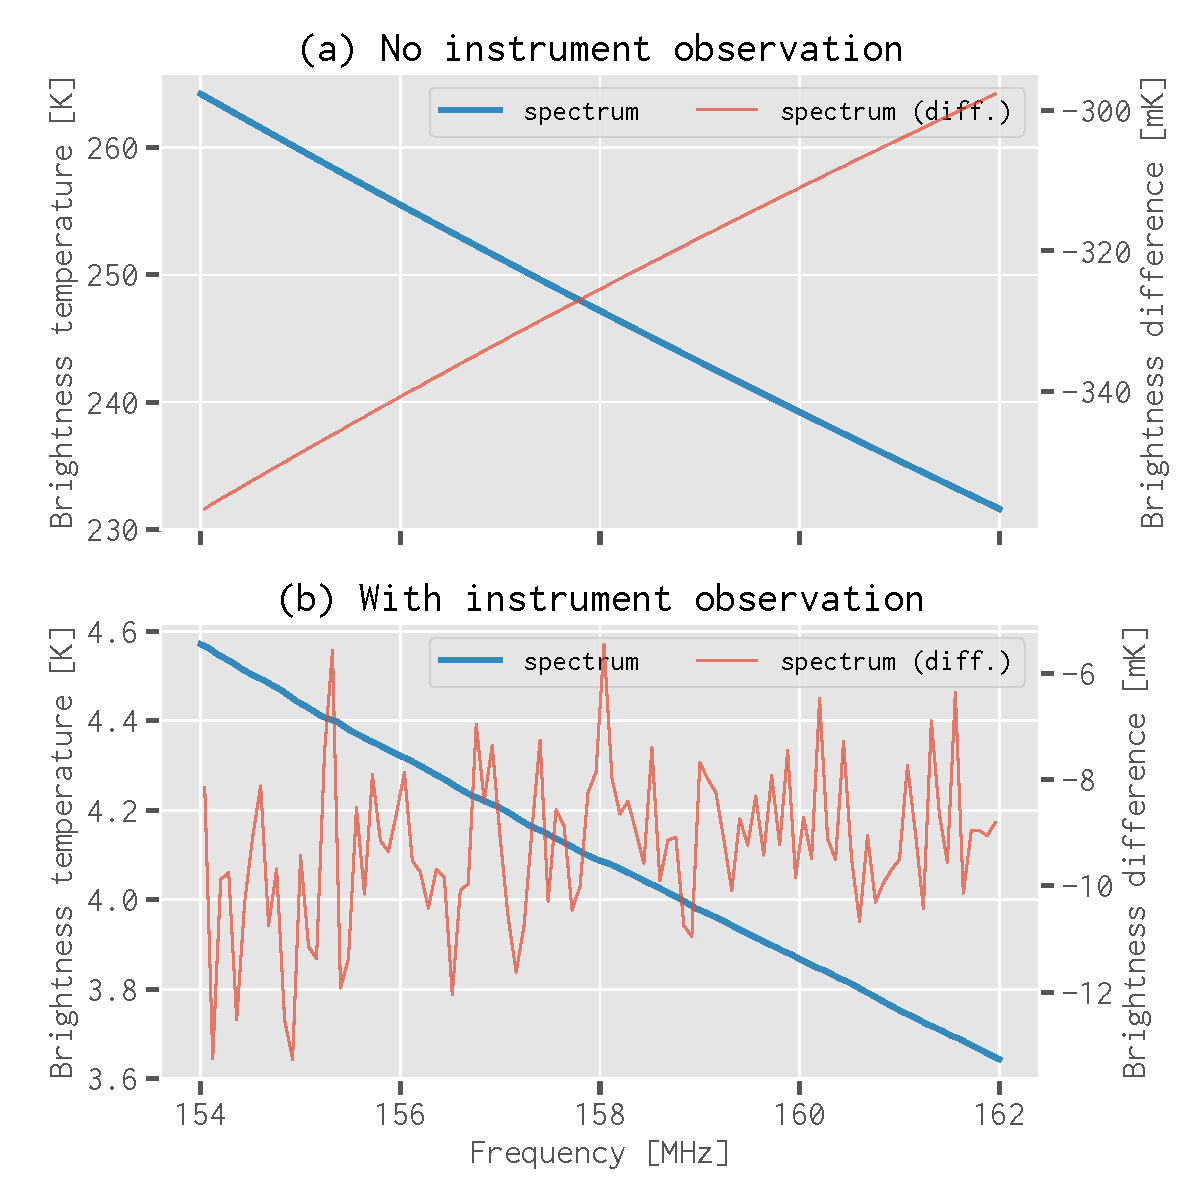
\includegraphics[width=\columnwidth]{simudata}
  \caption{\label{fig:simudata}%
    Example spectra (the bold blue lines) and the corresponding
    differential spectra (the thin red lines) for the foreground
    emission.
    The top and bottom panels show the cases without and with
    instrument observation, respectively.
  }
\end{figure}


%%----------------------------------------------------------------------
\subsection{Data preprocessing}
\label{sec:preprocessing}

The data set required by the CDAE consists of two parts:
(1) the input data (i.e., noisy EoR signal) that are the addition of
the EoR signal and the foreground emission, i.e.,
$\M{X}_{\R{in}} = \M{C}_{\R{eor}} + \M{C}_{\R{fg}}$;
(2) the `true' data that are the simulated EoR signal
(i.e., $\M{Y}_{\R{true}} = \M{C}_{\R{eor}}$)
and act as the goal of training the CDAE.

For the input data ($\M{X}_{\R{in}}$), we propose to apply the Fourier
Transform (FT) along the frequency dimension, which makes the EoR
signal more distinguishable from the foreground emission and thus
easier to learn by the CDAE (see also the comparison without applying
such FT to the data in \autoref{sec:noft}).
The Blackman-Nuttall window function is applied to suppress the
FT side-lobes caused by the sharp discontinuities at the ends
of the finite frequency band \citep[e.g.,][]{chapman2016}.
It is sufficient to keep only half the Fourier coefficients because
the data is real, thus the data of length 101 for one pixel in the
image cube are transformed to be 51 complex Fourier coefficients.
We excise the 6 coefficients of the lowest Fourier frequencies, which
have large values and are almost contributed by the spectral-smooth
foreground emission.
Since both the real and imaginary parts of the Fourier coefficients
are required to reconstruct the frequency-domain signal via inverse FT,
the real and imaginary parts are separated and concatenated into a new
vector of length 90.
Finally, the data are zero-centred and normalised to have unit variance.

The preprocessing steps for the `true' data ($\M{Y}_{\R{true}}$) are
similar but need minor adjustments.
After applying the FT, excising the 6 lowest Fourier components, and
concatenating the real and imaginary parts,
the data elements with value less than the 1$^{\R{th}}$ percentile or
greater than the 99$^{\R{th}}$ percentile are truncated, improving the
robustness of the data for training the CDAE.
Finally, the data are divided by the maximum absolute value of the
truncated data, constraining the value range to be $[-1, 1]$,
which renders the `tanh' activation function that has the same value
range appropriate for the output layer of the CDAE.


%%----------------------------------------------------------------------
\subsection{Training}
\label{sec:training}

The data set has 129,600 data points, i.e., the number of pixels of
the image cubes, and is randomly partitioned into the
training set ($S_{\R{tr}}$), validation set ($S_{\R{val}}$), and
test set ($S_{\R{test}}$) that account for 60, 20, and 20 per cent of
the whole data set, respectively [这是机器学习常用的切分比例].
The training set is used to train the parameters of the CDAE,
the validation set helps to determine the hyperparameters (e.g., the
number of layers and filters, the loss function),
while the test set is only employed to evaluate the performance of the
trained CDAE.

We implement the proposed CDAE using the popular \textsc{Keras}\footnote{%
  Keras: \url{https://keras.io} (version 2.2.0)}
framework \citep{keras} with the \textsc{TensorFlow}\footnote{%
TensorFlow: \url{https://www.tensorflow.org} (version 1.4.1)}
back end \citep{tensorflow} [这是目前最常用的编写神经网络的软件包].
The parameters of the Adam optimisation method are set to the default
values, i.e., learning rate being $\alpha = 0.001$, and
exponential decay rates for the first and second moment estimates being
$\beta_1 = 0.9$ and $\beta_2 = 0.999$, respectively \citep{kingma2015}.
The CDAE is trained on the training set ($S_{\R{tr}}$) with batch size
of 100 for 100 epochs so that the training loss converges.


%%----------------------------------------------------------------------
\subsection{Results}
\label{sec:results}

The training and validation losses together with the evaluation index
(i.e., the correlation coefficient) calculated on the validation set
($S_{\R{val}}$) during the training phase are shown in \autoref{fig:train}.
The steadily decreasing losses and increasing correlation coefficient
suggest that the CDAE is well trained without overfitting.
By evaluating on the test set ($S_{\R{test}}$), the trained CDAE
achieves excellent performance with a correlation coefficient of
$\rho_{\R{cdae}} = \num{0.969 +- 0.020}$.
As an example, \autoref{fig:result} illustrates the separated EoR signal
for one random pixel, exhibiting a correlation coefficient of
$\rho = 0.965$.
Consequently, our deep-learning-based method by using the CDAE is able
to overcome the frequency-dependent beam effects and accurately separate
the faint EoR signal in the presence of severe foreground contamination.

\begin{figure}
  \centering
  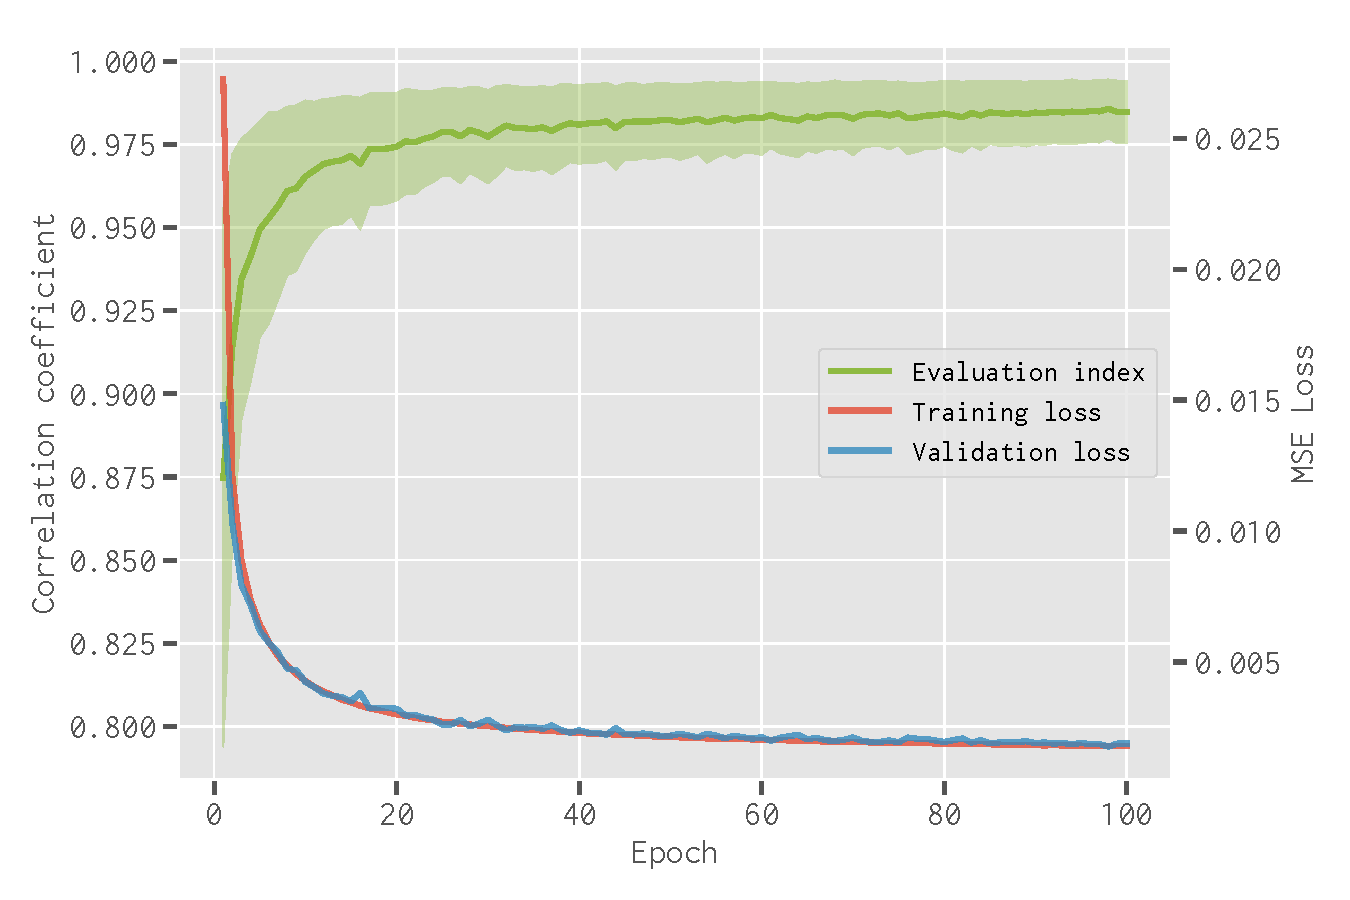
\includegraphics[width=\columnwidth]{cdae-train}
  \caption{\label{fig:train}%
    The training loss (the red line), validation loss (the blue line),
    and correlation coefficient calculated on the validation set
    $S_{\R{val}}$ (the green line with the shaded region representing
    the standard deviation) during the training of the CDAE.
  }
\end{figure}

\begin{figure}
  \centering
  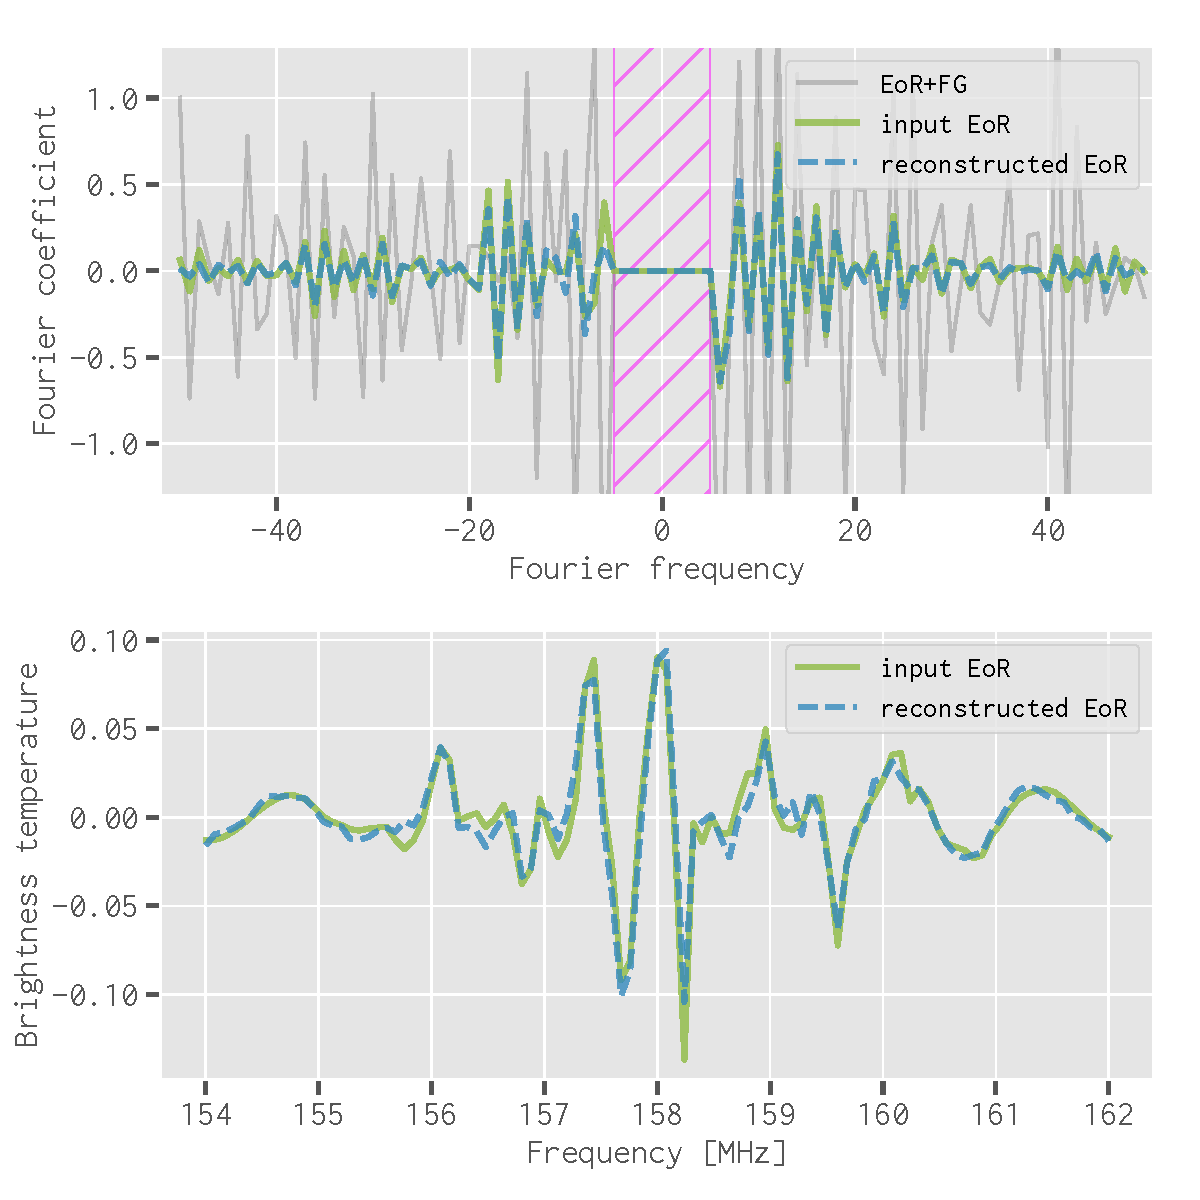
\includegraphics[width=\columnwidth]{eor-result}
  \caption{\label{fig:result}%
    An example of the EoR signal separated by the trained CDAE for one
    random pixel.
    \textbf{(top)} The `true' EoR signal (the solid green line) and the
    separated EoR signal (the dashed blue line) in the Fourier domain
    where the CDAE training is performed.
    The grey line represents the input data for the CDAE that contains
    both the EoR signal and the foreground emission.
    The magenta hatched region marks the excised Fourier coefficients
    in data preprocessing.
    \textbf{(bottom)} The `true' EoR signal (the solid green line) and
    the separated EoR signal (the dashed blue line) transformed back to
    the observing frequency domain.
  }
\end{figure}
  }
\end{figure}


%%----------------------------------------------------------------------
\subsection{Comparison}
\label{sec:comparison}

In order to better demonstrate the excellent performance of our proposed
method, we carry out a comparison between our method and the traditional
polynomial fitting method.
Using the same data set simulated in \autoref{sec:data}, for each pixel
in the image cube of the addition of the EoR signal and the foreground
emission, a low-order polynomial is fitted along the frequency
dimension, the fitted value of which is then subtracted to uncover the
EoR signal.
We have tested polynomials of order from 2 (quadratic) to 5 (quintic),
and find that the quartic polynomial (order of 4) can give the
relatively best result.
However, the correlation coefficient calculated for the separated EoR
signal in such case is only $\rho_{\R{pfit}} = \num{0.241 +- 0.103}$,
which is rather small and indicates that the polynomial fitting method
performs very poor in separating the EoR signal.
As illustrated in \autoref{fig:simudata}, the complicated instrumental
effects seriously damage the spectral smoothness of the foreground
emission, causing rapid fluctuations of similar strength as or even
stronger than the EoR signal, therefore, it is unsurprising that the
polynomial fitting method gives very poor results.
On the contrary, our deep-learning-based method is superior and
by far outperforms the traditional polynomial fitting method.


%%======================================================================
\section{Conclusions}
\label{sec:conclusions}

We have demonstrated to use the CDAE to separate the faint EoR signal
that is buried in the overwhelming foreground contamination with the
complicated instrumental effects taken into account.
The proposed CDAE, which consists of a 7-layer encoder, a 7-layer
decoder, and one output layer, is trained on the simulated SKA images
and achieves excellent performance that is by far better than the
traditional polynomial fitting method.
In conclusion, our deep-learning-based method is able to accurately
separate the faint EoR signal in the presence of severe foreground
contamination and complicated instrumental effects.
In addition, the proposed CDAE is simple but powerful, exhibiting the
great potential of deep-learning-based methods to play an important
role in forthcoming EoR experiments.


%%======================================================================
\section*{Acknowledgements}

This work is supported by
the Ministry of Science and Technology of China
(grant Nos. 2018YFA0404601, 2017YFF0210903),
and the National Natural Science Foundation of China
(grant Nos. 11433002, 11621303, 11835009, 61371147).


%%======================================================================
%% References

\bibliographystyle{mnras}
\bibliography{references}


%%======================================================================
%% Appendix

% \appendix


%%======================================================================
% Don't change these lines
\bsp	% typesetting comment
\label{lastpage}
\end{document}

%% EOF
